\documentclass{beamer}

\usepackage[spanish]{babel}
\selectlanguage{spanish}
\usepackage[utf8]{inputenc}
\usepackage{graphicx,hyperref,ru,url,bm}

\setbeamertemplate{caption}{\raggedright\insertcaption\par}

\def\realR{\mathbb{R}} % Defines the way to use real numbers symbol R.

% The title of the presentation:
%  - first a short version which is visible at the bottom of each slide;
%  - second the full title shown on the title slide;
\title[Espacios Tangentes]{
    Espacios Tangentes}

% Optional: a subtitle to be dispalyed on the title slide
\subtitle{El concepto abstracto de curva en $\realR^{2}$ y variedad en $\realR^{n}$}

% The author(s) of the presentation:
%  - again first a short version to be displayed at the bottom;
%  - next the full list of authors, which may include contact information;
\author[Joaquín González Cervantes]{
  Joaquín González Cervantes \\\medskip
  {\small \url{joaquin@yandex.com}}}

% The institute:
%  - to start the name of the university as displayed on the top of each slide
%    this can be adjusted such that you can also create a Dutch version
%  - next the institute information as displayed on the title slide
\institute[Universidad de Guadalajara]{}

% Add a date and possibly the name of the event to the slides
%  - again first a short version to be shown at the bottom of each slide
%  - second the full date and event name for the title slide
\date[\today]{
   \today}

\begin{document}

\begin{frame}
  \titlepage
\end{frame}

% Section titles are shown in at the top of the slides with the current section 
% highlighted. Note that the number of sections determines the size of the top 
% bar, and hence the university name and logo. If you do not add any sections 
% they will not be visible.
\section{Introducción}

\begin{frame}
\frametitle{¿De qué trata?}
  \begin{block}{}
    \begin{itemize}
        \item Definir el concepto general de curva en $\realR^{2}$ y su espacio tangente.
        \item Una breve introducción al concepto de variedad y su espacio tangente.
    \end{itemize}
  \end{block}
\end{frame}

\begin{frame}
\begin{columns}
\column{0.5\textwidth}
    \begin{center}
        \includegraphics[scale=0.25]{curva-suave}
    \end{center}
\column{0.5\textwidth}
    \begin{center}
        \includegraphics[scale=0.35]{curva-no-suave}
    \end{center}
\end{columns}
\end{frame}

\begin{frame}
  \begin{block}{Estrategia}
    \begin{itemize}
        \item Empezar con curvas suaves parametrizadas en $\realR^{2}$ y calcular su espacio tangente.
        \item Generalizar la definición de curva en $\realR^{2}$.
        \item Con nuestra nueva definición, determinar el espacio tangente.
        \item Teorema de la función implícita para funciones $F(x,y) = 0$.
        \item Conectar lo anterior con el concepto de curva en $\realR^{n}$.
    \end{itemize}
  \end{block}
\end{frame}

\begin{frame}
    \frametitle{Antes que el vector}
    \includegraphics[width=\textwidth]{../gfx/cardano-leibniz}
\end{frame}

\begin{frame}
    \includegraphics[width=\textwidth]{../gfx/newton-wessel}
\end{frame}

\begin{frame}
    \begin{center}
        \includegraphics[width=0.6\textwidth]{../gfx/gauss-frame}
    \end{center}
\end{frame}

\begin{frame}
    \frametitle{La ambición de Hamilton}
    \begin{columns}
    \column{0.5\textwidth}
        \begin{center}
            \begin{figure}
            \includegraphics[scale=0.4]{../gfx/hamilton}
                \caption{William Rowan Hamilton (1843)}
            \end{figure}
        \end{center}
    \column{0.5\textwidth}
    \end{columns}
\end{frame}

\begin{frame}
    \frametitle{La ambición de Hamilton}
    \begin{columns}
    \column{0.5\textwidth}
        \begin{center}
            \begin{figure}
            \includegraphics[scale=0.4]{../gfx/hamilton}
                \caption{William Rowan Hamilton (1843)}
            \end{figure}
        \end{center}
    \column{0.5\textwidth}
        Cuaternión:
        \begin{eqnarray*}
            Q &=& a + x\bm{i} + y\bm{j} + z\bm{k}
        \end{eqnarray*}
    \end{columns}
\end{frame}

\begin{frame}
    \frametitle{La ambición de Hamilton}
    \begin{columns}
    \column{0.5\textwidth}
        \begin{center}
            \begin{figure}
            \includegraphics[scale=0.4]{../gfx/hamilton}
                \caption{William Rowan Hamilton (1843)}
            \end{figure}
        \end{center}
    \column{0.5\textwidth}
       Cuaternión:
       \begin{eqnarray*}
           Q &=& a + x\bm{i} + y\bm{j} + z\bm{k} \\
             &=& SQ + VQ
       \end{eqnarray*}
    \end{columns}
\end{frame}

\begin{frame}
    \frametitle{La ambición de Hamilton}
    \begin{columns}
    \column{0.5\textwidth}
        \begin{center}
            \begin{figure}
            \includegraphics[scale=0.4]{../gfx/hamilton}
                \caption{William Rowan Hamilton (1843)}
            \end{figure}
        \end{center}
    \column{0.5\textwidth} 
       Cuaternión:
       \begin{eqnarray*}
           Q &=& a + x\bm{i} + y\bm{j} + z\bm{k} \\
           &=& SQ + VQ \\ \\
           Q_{1}Q_{2} &=& -Q_{2}Q_{1}  
       \end{eqnarray*}
    \end{columns}
\end{frame}

\begin{frame}
    \frametitle{Más sistemas vectoriales}
    \begin{columns}
    \column{0.5\textwidth}
        \begin{center}
            \begin{figure}
            \includegraphics[scale=0.4]{../gfx/grassmann}
                \caption{Hermann Grassmann (1844)}
            \end{figure}
        \end{center}
    \column{0.5\textwidth} 
        \includegraphics[width=\textwidth]{../gfx/grassmann-book}
    \end{columns}
\end{frame}

\begin{frame}
    \begin{columns}
    \column{0.5\textwidth}
        \begin{center}
            \begin{figure}
            \includegraphics[scale=0.4]{../gfx/gibbs}
                \caption{Josiah Willard Gibbs (1881)}
            \end{figure}
        \end{center}
    \column{0.5\textwidth} 
       \begin{eqnarray*}
           \alpha . \beta &=& \beta . \alpha \quad \text{Gibbs} \\
           S\alpha\beta &=& S\beta\alpha \quad \text{Tait} \\
           \alpha \times \beta &=& -\beta \times \alpha \quad \text{Gibbs} \\  
           V\alpha\beta &=& -V\beta\alpha \quad \text{Tait} \\  
       \end{eqnarray*}
    \end{columns}
\end{frame}

\section{pronto ...}

\begin{frame}
\end{frame}

\section{pronto ...}
\begin{frame}
\frametitle{pronto ...}

\end{frame}

\section{pronto ...}
\begin{frame}
\frametitle{pronto ...}

\end{frame}

\end{document}
